\newcommand{\VS}{\vspace{6pt}}
\newcommand{\vt}[1]{\vec{#1}}

\chapter{Dynamic Step} % Main chapter title

\label{Chapter1} % For referencing the chapter elsewhere, use \ref{Chapter1} 

%----------------------------------------------------------------------------------------

This modification is based on the constant step variant of the SVM-RFE algorithm, however, instead of using some constant number as the step in each iteration we calculate that number dynamically. The most straightforward way to do this is by using a percentage. Another possibility is to let the model score influence this percentage.

\section{Description and reasoning}
\label{sec:dynamicStep.desc}

The percentage is a hyperparameter. It is used within every iteration to select a number of the first ranked features. A constant step has already been used in pract\-ice, but it is expected that this method will be significantly faster without effecting the accuracy performance, or even improving it.

The reasoning behind this is that when you have many features for which you only want to select a very small subset, the required amount of iterations will be of lineal complexity on the amount of features, however, by using a percentage, we get a logarithmic complexity.

Other similar modifications are also found in the literature, including using the square root of the remaining features \texttt{SQRT-RFE}, an entropy based function \texttt{E-RFE}, or \texttt{RFE-Annealing} which sets the step at $|\vt{s}| \frac{1}{i+1}$, thus, changing the percentage each iteration (\cite{ding_improving_2006}).

\iffalse
That is, the amount of features eliminated "$r$" at $j$-th iteration is the summation of the amount of features eliminated each iteration, i.e. $np^i$:

\begin{equation}\label{eq:dynamicStep1}
    r = \sum_{i = 1}^{j}{(np^i)} 
\end{equation}

It may be more interesting to see complexity as in the amount of iterations re\-quired to eliminate $r$ features, it can be derived from equation \ref{eq:dynamicStep1} as follows:

\begin{align*}
    r &= n \sum_{i = 1}^{j}{p^i} = n \sum_{i = 0}^{j-1}{(p^i)} - n + np^j \\
    \frac{r}{n} &= \frac{1-p^j}{1-p} - 1 + p^j \\
    \frac{r}{n} &= \frac{(1-p^j) - (1-p) + (1-p)p^j}{1-p}\\
    \frac{(1-p)r}{n} &= (1-p^j) - (1-p) + (p^j-p^{j+1})\\
    \frac{(1-p)r}{n} &= 1 -p^j -1 + p + p^j - p^{j+1}\\
    \frac{(1-p)r}{n} &= p - p^{j+1}\\
    - \frac{(1-p)r}{n} + p &= p^{j+1}\\
    \log_{p} \left( - \frac{(1-p)r - np}{n} \right) &= \log_{p} (p^{j+1})\\
    \log_{p} \left( - \frac{(1-p)r - np}{n} \right) &= j + 1\\
    \log_{1/p} \left( - \frac{n}{(1-p)r} + 1/p \right) &= j + 1\\
\end{align*}
\fi

We assume that, the bigger the step in each iteration, the worse the performance of the final selection. However, since we're selecting the worst variables first, se\-lect\-ing more of them at once shouldn't affect performance because they would have been selected anyway with height probability in the following iterations. The fewer the iterations remaining, the riskier it becomes selecting multiple variables at once, and thus a smaller step is beneficial.

\section{Pseudocode formalization}

\textbf{Definitions:}

\begin{itemize}
    \item $X_0 = [\vt{x_0}, \vt{x_1}, \dotsc, \vt{x_k}]^T$ list of observations.
    \item $\vt{y} = [y_1, y_2, \dotsc, y_k]^T$ list of labels.
\end{itemize}

\begin{algorithm}[H]
    \DontPrintSemicolon
      \KwInput{$p$ \tcp*{p = percentage, $0 \le p \le 1$}}
      \KwOutput{$\vt{r}$}
      \KwData{$X_0,\vt{y}$}
      $\vt{s} = [1,2, \dotsc, n]$ \tcp*{subset of surviving features}
      $\vt{r} = []$ \tcp*{feature ranked list} 
      \While{$|\vt{s}| > 0$}
        {
            \tcc*[h]{Restrict training examples to good feature indices}\\
            $X=X_0(:,\vt{s})$\VS

            \tcc*[h]{Train the classifier}\\
            $\vt{\alpha} = \texttt{SVM-train(} X, y \texttt{)}$\VS

            \tcc*[h]{Compute the weight vector of dimension length $|\vt{s}|$}\\
            $\vt{w} = \sum_k{\vt{\alpha_k} \vt{y_k} \vt{x_k}}$\VS

            \tcc*[h]{Compute the ranking criteria}\\
            $\vt{c} = [(w_i)^2 \text{ for all $i$}]$\VS

            \tcc*[h]{Compute $t$ based on the percentage}\\
            $t = p|\vt{s}|$\VS

            \tcc*[h]{Find the $t$ features with the smallest ranking criterion}\\
            $\vt{f} = \texttt{argsort}(\vt{c})(\ :t)$\VS

            \tcc*[h]{Update the feature ranking list}\\
            $\vt{r} = [\vt{s}(\vt{f}), ...\vt{r}]$\VS

            \tcc*[h]{Eliminate the features with the $t$ smallest ranking criterion}\\
            $\vt{s} = [[...\vt{s}(1:f_i - 1), ...\vt{s}(f_i + 1:|\vt{s}|)]$ for all $i]$
        }
    \caption{SVM-RFE with DynamicStep}
\end{algorithm}

\section{Results}

\subsection{Initial Analysis with Madelon}

We've initially run some tests to find how hard it is for the SVM-RFE algorithm to work with it. 

The first test consists on simply doing a random feature selection and plotting the accuracy for the training and test splits (Figure \ref{fig:dynamicStep.madelon.base}). This random selection algorithm will allow us to make comparisons with other feature selection algorithms to determine whether they work or not. Because we're using the average of many random selection experiments, the curve it produces should be always worse than that of any other working selection algorithm. It is expected that it will produce a somewhat linear function with accuracy dropping consistently when the amount of features selected is reduced.

\begin{figure}[H]
    \centering
    \begin{subfigure}[b]{0.4\linewidth}
        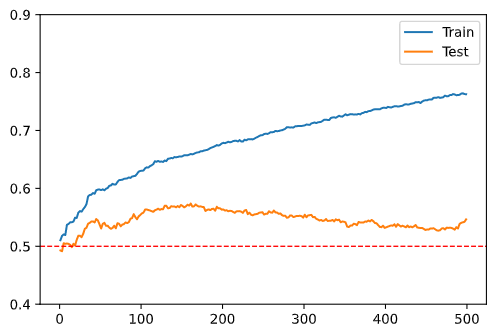
\includegraphics[width=\linewidth]{img/madelon-random-c_1}
        \subcaption*{$C=1$}
    \end{subfigure}
    \begin{subfigure}[b]{0.4\linewidth}
        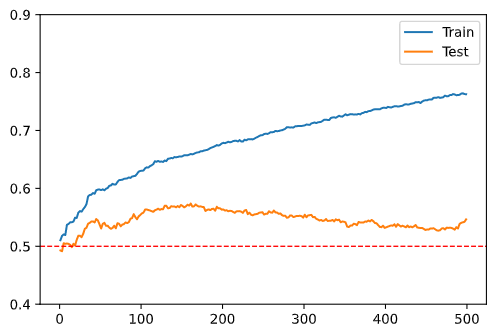
\includegraphics[width=\linewidth]{img/madelon-random-c_1}
        \subcaption*{$C=10^3$}
    \end{subfigure}
    \caption{Accuracy of an SVM classifier with a random feature selection with the Madelon dataset.}
    \label{fig:dynamicStep.madelon.base}
\end{figure}

The results of this test are a bit unexpected. Although the training accuracy behaves as expected, the test accuracy is way too low for even the case where all features are used (0.55). Reducing the amount of features, even randomly, produces a slight increase in the test accuracy. This is a fine example of the effects of the curse of dimensionality, on how even a random selection, which should produce consistently worse models the less amount of features it has, ends up producing better ones simply because there are fewer features with independence on how the feature selection is made.

We've performed a second test to see if the regularization parameter has any effect and can be of any help in trying to reduce overfitting (Figure \ref{fig:dynamicStep.madelon.reg}).

\begin{figure}[h]
    \centering
    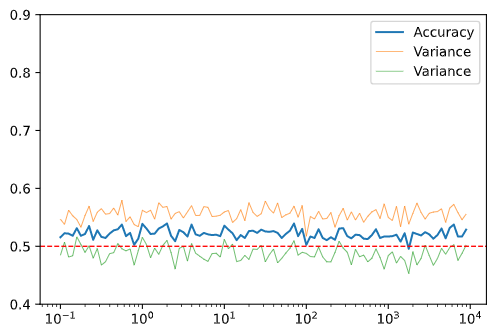
\includegraphics[width=0.4\linewidth]{img/madelon-cv-c}
    \caption{Test accuracy mean of SVM classifier with 10-fold cross-validation using all features for multiple values of C.}
    \label{fig:dynamicStep.madelon.reg}
\end{figure}

As the plot indicates, no value of the regularization parameter helps improve the performance. These poor results suggest that the dataset is not linearly separable and thus is producing huge amounts of overfitting in all cases, but, how does this affect SVM-RFE?

To see how SVM-RFE performs under these conditions we've designed an ex\-periment very similar to that used in random selection, although instead of using 10 random selections we've used cross-validation to take the mean. In this experiment we also use a constant step of 10 for performance reasons, see Figure \ref{fig:dynamicStep.madelon.step10}.

\begin{figure}[h]
    \centering
    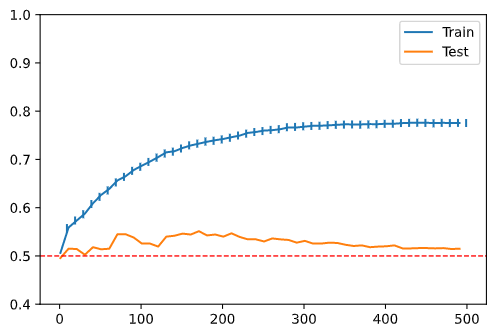
\includegraphics[width=0.4\linewidth]{img/madelon-svmrfe-step-s_10}
    \caption{Mean accuracy using 20-fold CV of an SVM classifier with SVM-RFE selection of the Madelon dataset.}
    \label{fig:dynamicStep.madelon.step10}
\end{figure}

Comparing this plot with that of the random selection we can see that the results are quite disappointing. Although SVM-RFE does improve the performance on the training data, the test performance remains the same. With this we can conclude that SVM-RFE using a lineal kernel does not work well on this specific dataset, and thus, no matter the step strategy used, the results will all be quite bad. 

We have also checked how does SVM-RFE perform if we use a dynamic step strategy (Figure \ref{fig:dynamicStep.madelon.dstep}), but no significant difference is appreciated.

\begin{figure}[H]
    \centering
    \begin{subfigure}[b]{0.4\linewidth}
        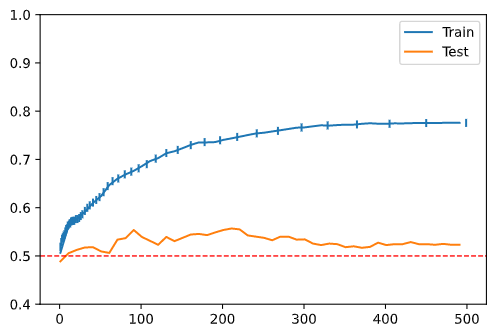
\includegraphics[width=\linewidth]{img/madelon-svmrfe-dstep-p_01.png}
        \subcaption*{10\%, 52 iterations, stop at 0}
    \end{subfigure}
    \begin{subfigure}[b]{0.4\linewidth}
        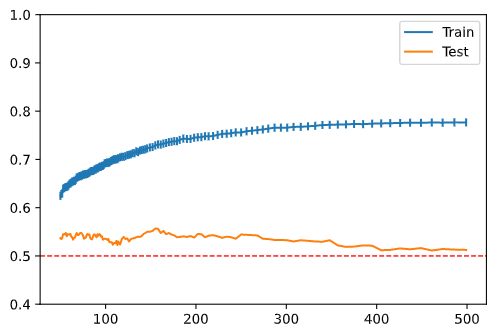
\includegraphics[width=\linewidth]{img/madelon-svmrfe-dstep-p_003.png}
        \subcaption*{3\%, 136 iterations, stop at 50}
    \end{subfigure}
    \caption{Mean accuracy using 20-fold CV of an SVM classifier with SVM-RFE selection using dynamic step of the Madelon dataset.}
    \label{fig:dynamicStep.madelon.dstep}
\end{figure}


This is a problem. We've initially wanted to use the Madelon dataset to do our experiments, but these results show that the dataset in not adequate for a linear classifier. Thus, we've decided to use simpler artificially generated datasets for this experiment and come back to the Madelon dataset later on with other extensions of the SVM-RFE algorithm.

\subsection{Initial Analysis with artificially generated data}

To generate the dataset we've used the \textit{make\_classification} function of the \texttt{Sklearn} library. We've created a dataset with 300 features, 50 of which are informative. Ideally, a perfect feature selection algorithm should be able to produce a peak test accuracy at the exact amount of informative features or less.

Similar to the experiments descried before, we've performed random selection and SVM-RFE. Here tough, we also make a comparison with different values of the step to see how it effects the actual performance of the selection. In the particular case where the step is equal to the amount of features this is no longer SVM-RFE but a filter method based on SVM (one single iteration).

\begin{figure}[H]
    \centering
    \begin{subfigure}[b]{0.4\linewidth}
        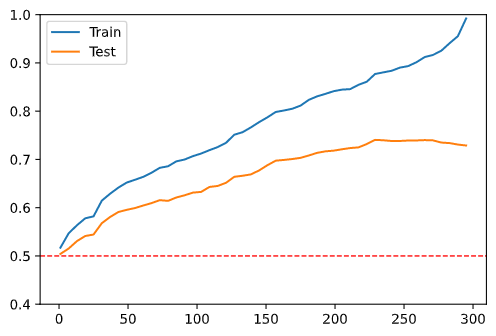
\includegraphics[width=\linewidth]{img/vanilla300-random.png}
        \subcaption*{\textbf{A.} Random selection}
    \end{subfigure}
    \begin{subfigure}[b]{0.4\linewidth}
        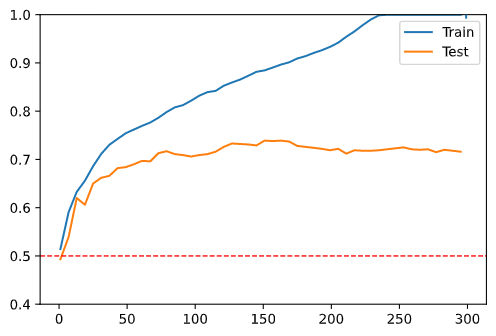
\includegraphics[width=\linewidth]{img/vanilla300-svmrfe-s300.png}
        \subcaption*{\textbf{B.} SVM-based filter method, step = 300}
    \end{subfigure}
    \begin{subfigure}[b]{0.4\linewidth}
        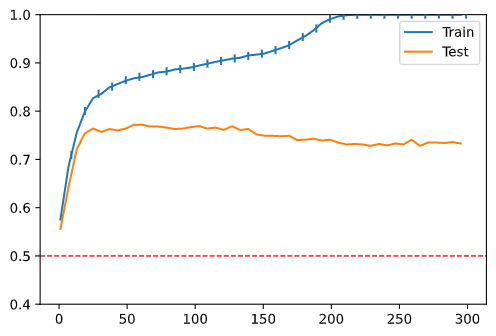
\includegraphics[width=\linewidth]{img/vanilla300-svmrfe-s10.png}
        \subcaption*{\textbf{C.} SVM-RFE, step = 10}
    \end{subfigure}
    \begin{subfigure}[b]{0.4\linewidth}
        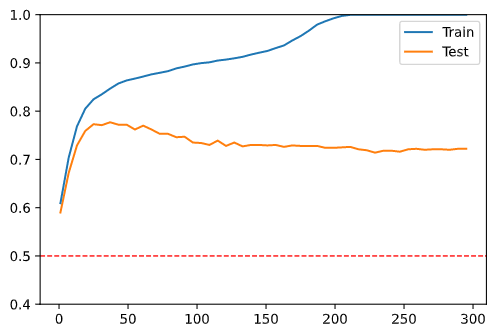
\includegraphics[width=\linewidth]{img/vanilla300-svmrfe.png}
        \subcaption*{\textbf{D.} SVM-RFE, step = 1}
    \end{subfigure}
    \caption{Mean accuracy using 20-fold CV of an SVM classifier with different selection methods.}
    \label{fig:dynamicStep.vanilla.comp}
\end{figure}

From this analysis we conclude that SVM-RFE works well on this dataset. We also verify, by comparing plots \textbf{B} and \textbf{C}, our previous assumption that the more iterations (smaller step) the better the accuracy. This relationship, however, doesn't seem to be lineal, as the same effect can not be appreciated when comparing plots \textbf{C} and \textbf{D}.

Notice that when evaluating the performance of a feature selection algorithm two variables must be considered, one is accuracy performance and the other is amount of features. A selection with a great accuracy but a lot of features may not be as good as a section with a decent accuracy and only a handful of features. That is, we want to maximize accuracy while minimizing amount of features. These two variables do not operate on the same range, and it can even be the case that the importance of one over the other is problem-dependent. This makes comparing multiple instances hard, this is why are comparing pairs of plots instead of simply a pair of values.

\subsection{Dynamic Step vs Constant Step}

Based on our assumptions, dynamic step can never beat in accuracy performance a constant step of one. Beating constant steps bigger than 1 should theoretically be possible when the amount of features is huge, since at some point the specific step used will be smaller than the constant, and there an improvement may be found. For our specific dataset of 300 features however, no such improvement was found, likely because the amount of features was insufficient, but also because of the no linearity of the stated property.

Rather than for improving accuracy, dynamic step is more useful for improving computational cost. Because each iteration reduces the amount of features, training the SVM will be faster with dynamic step even if the same amount of iterations are used, since there will be more iterations using fewer features in the dynamic step case.

This same mechanic does not apply only to using percentages, the other methods stated at section \ref{sec:dynamicStep.desc} follow the same logic. In Figure \ref{fig:dynamicStep.compare} you can see a comparison of dynamic step methods. Although all of them draw some kind of curve, they don't use the same shape, and thus can produce slightly different performance results using the same amount of iterations. The time cost of the methods can be estimated as the area under the curve.

\begin{figure}[h]
    \centering
    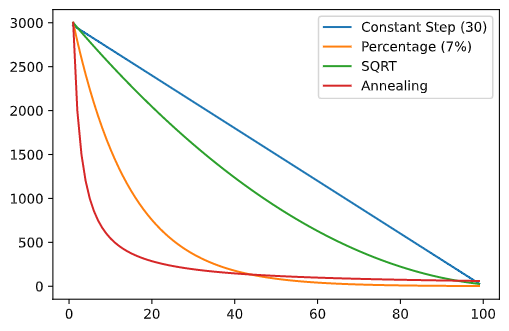
\includegraphics[width=0.4\linewidth]{img/comparetimes.png}
    \caption{Amount of features remaining (vertical axis) at each iteration (horizontal axis).}
    \label{fig:dynamicStep.compare}
\end{figure}

Experimentally we confirm our results and see that using a percentage is faster compared to a constant step, without reducing its accuracy. The following table summarizes the time cost for various experiments. The SVM-RFE time shown is the mean of the times of every fold used during cross-validation.

\begin{table}[h]
    \centering
    \begin{tabular}{l r r r}
    \toprule
    \tabhead{Strategy} & \tabhead{Iterations} & \tabhead{Time} & \tabhead{Total Time} \\
    \midrule
    Constant & 60 & 29.16s & 00:02:36\\
    Constant & 30 & 15.90s & 00:02:00\\
    Constant &  6 & 4.43s  & 00:01:29\\
    Constant &  3 & 2.74s  & 00:01:22\\
    Percentage & 47 & 7.03s & 00:01:29\\
    Percentage & 26 & 3.83s & 00:01:17\\
    Percentage & 10 & 2.59s & 00:01:13\\
    \bottomrule\\
    \end{tabular}
    \caption{Time costs for various experiments.}
    \label{tab:dynamicStep.times}
\end{table}

Notice that although one could think that the smaller the area under the curve the better, and it is true when it comes to time costs, a very pronounced curve would imply a very big initial step, this can result in a drop in accuracy performance in the very first iterations that can not be restored later on even with a step of 1. This is specially important for the annealing method, since it chooses a 50\% percentage in the very first iteration. How much acute the curve can be without producing a drop in accuracy depends on the dataset, specifically on the amount of informative features. Thus, introducing a hyperparameter to specify the sharpness of the curve may be useful. The percentage approx already has this hyperparameter by default, but introducing such parameter in the other methods is also trivial. Another option would be to further customize the curve by introducing minimum and maximum steps.

Finally, one last parameter that may be of relevance is the stop value. If the amount of informative variables is known, it doesn't make sense to perform many iterations on selections so small that the performance has already dropped, instead it may make more sense to increase the amount of iterations the closer you get to the amount of informative variables. This effect can be seen in Figure \ref{fig:dynamicStep.vanilla.stop}.

\begin{figure}[H]
    \centering
    \begin{subfigure}[b]{0.4\linewidth}
        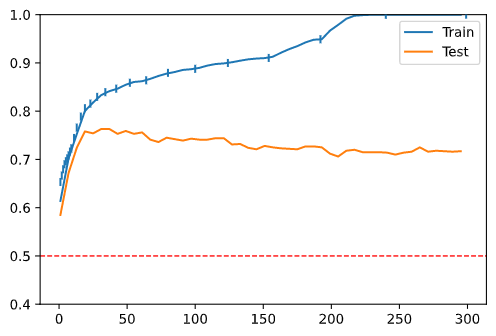
\includegraphics[width=\linewidth]{img/vanilla300-svmrfe-stopA.png}
        \subcaption*{2\%, 26 iterations, stop at 0}
    \end{subfigure}
    \begin{subfigure}[b]{0.4\linewidth}
        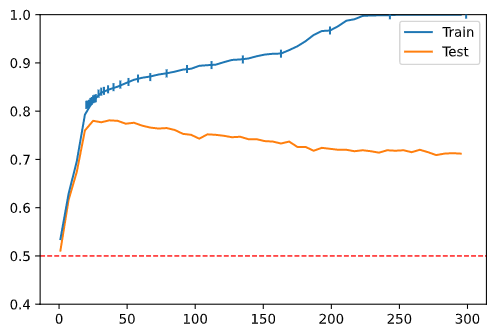
\includegraphics[width=\linewidth]{img/vanilla300-svmrfe-stopB.png}
        \subcaption*{2\%, 25 iterations, stop at 20}
    \end{subfigure}
    \caption{Comparison of the dynamic step behavior with and without using a stop parameter.}
    \label{fig:dynamicStep.vanilla.stop}
\end{figure}

\subsection{Annotations}

\begin{itemize}
    \item The Cross Validation procedure has been implemented by hand and par\-al\-lelized.
    \item How do I know which method is better?
    \item How do I measure how good some method is (accuracy vs selection size)? Mathematically.
    \item Should I do hyperparameter search (of C) also here?
    \item Explain why plotting takes so much time.
    \item Should the percentage really be a hyperparameter? Annealing and Square Root do not, and it doesn't make much of a difference anyways?
    \item The complexity of SVM seems to be $O(\max(n, d) \min(n, d)^2)$. \\ If dimensions > nº observations: $O(dn^2)$. \\ Otherwise: $O(nd^2)$.
\end{itemize}